\section{Rozstrzygalność problemów}
Rozstrzygalność rozumiemy następująco:
\begin{align*}
& \ \: \rec - \text{rozstrzygalne} \\
& \left.
\begin{array}{l}
\re - \text{częściowo rozstrzygalne} \\
\overline{\re} - \text{nierozstrzygalne}
\end{array}
\right\} \text{nierozstrzygalne}
\end{align*}

\subsection{Język diagonalny}
Definiujemy język diagonalny
\[ L_D = \set{w_i \in \Sigma_i^*: w_i \notin L(M_i)} \]
\begin{theorem}
    \( L_D \notin \rec \)
\end{theorem}
\begin{proof}
    Nie wprost, załóżmy, że \( L_D \in \rec \), istnieje więc maszyna \(M_i\), która go rozstrzyga.
    \begin{itemize}
        \item Jeśli \( w_i \in L(M_i) \), to \( w_i \notin L_D = L(M_i) \)
        \item Jeśli \( w_i \notin L(M_i) \), to \( w_i \notin L_D = L(M_i) \)
    \end{itemize}
\end{proof}

\subsection{Język uniwersalny}
\[ L_u = \set{\langle M \rangle, w: w \in \Sigma^*, w \in L(M)} \]
\begin{theorem}
    \(L_U \in \re\)
\end{theorem}
\begin{proof}
Konstruujemy trzytaśmową maszynę rozstrzygającą \(L_U\):
\begin{enumerate}
    \item Wydziel kod maszyny \(\langle M \rangle\) i słowo \(w \in \Sigma^*\).
    \item Symuluj \(M\) na \(w\) przez \(i\) kroków
    \begin{enumerate}
        \item Jeżeli \(M\) akceptuje \(w\) po \(i\) krokach to zatrzymaj się i zwróć tak
        \item W przeciwnym przypadku przypisz \( i = i+1 \) i wróć do 2(a).
    \end{enumerate}
\end{enumerate}
Skonstruowana w dowodzie maszyna to uniwersalna maszyna Turinga \(M_U\), \( L_U = L(M_U) \). Taka maszyna może i umie zasymulować każdą inną maszynę Turinga.
\end{proof}

\begin{theorem}
    \(L_U \notin \rec\)
\end{theorem}
To wynika z Twierdzenia Rice'a, które już niedługo :)

\subsection{(Nie)pustość języków}
\begin{align*}
    & L_e = \set{\langle M \rangle : L(M) = \emptyset} \\
    & L_{ne} = \set{\langle M \rangle : L(M) \neq \emptyset}
\end{align*}

\begin{theorem}
    \( L_{ne} \in \re \)
\end{theorem}
\begin{proof}
    Konstruujemy maszynę rozpoznającą \(L_{ne}\): \\
    \begin{minipage}{0.6\linewidth}   
        \begin{enumerate}
            \item Wczytaj \(\langle M \rangle\) i sprawdź, czy jest poprawnym \\ kodem.
            \item Symuluj \(j\) kroków maszyny \(M\) na \(i\)-tym słowie \\ wg porządku \((i,j)\), zaczynając od \((0,0)\).
            \item Jeśli \(M\) akceptuje słowo, to zaakceptuj \(\langle M \rangle\).
        \end{enumerate}
    \end{minipage}
    \begin{minipage}{0.4\linewidth}
    \begin{figure}[H]
        \centering
        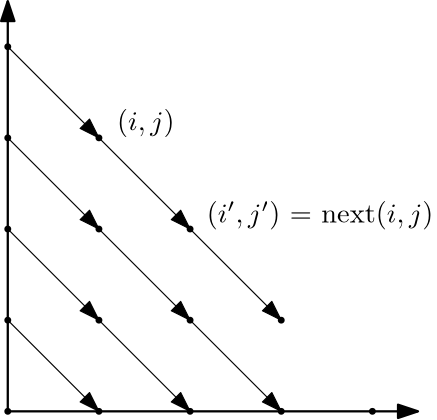
\includegraphics[width=0.65\linewidth]{img/Lne.png}
    \end{figure}   
    \end{minipage}
\end{proof}

\begin{theorem}
    \( L_e \notin \re \)
\end{theorem}
\begin{proof}
    Załóżmy dla dowodu nie wprost, że \( L_e \in \rec \). Konstruujemy maszynę \(N\) z własnością STOP, która akceptuje wszystko, jeśli \(w \in L(M)\) i nic wpp.

    Maszyna \(N\) rozpoznaje \(L_U \in \re\), co prowadzi do sprzeczności. \\

    Zatem \( L_e \notin \rec \), a ponieważ \( L_{ne} = \Sigma^* \setminus L_e \in \re \), to \( L_e \) jest całkiem nierozstrzygalny.
\end{proof}

\subsection{Rekurencyjność języków}
\begin{align*}
    & L_{rec} = \set{\langle M \rangle : L(M) \in \rec} \\
    & L_{nrec} = \set{\langle M \rangle : L(M) \notin \rec}
\end{align*}
Przykład nierozstrzygalnych języków,    których suma \( L_{rec} \cup L_{nrec} = \set{\langle M \rangle} \) jest rozstrzygalna.

\begin{theorem}
    \( L_{rec} \notin \re \)
\end{theorem}
\begin{proof}
     Załóżmy dla dowodu nie wprost, że \( L_{rec} \in \re \). Konstruujemy maszynę \(N\):
    \begin{figure}[H]
        \centering
        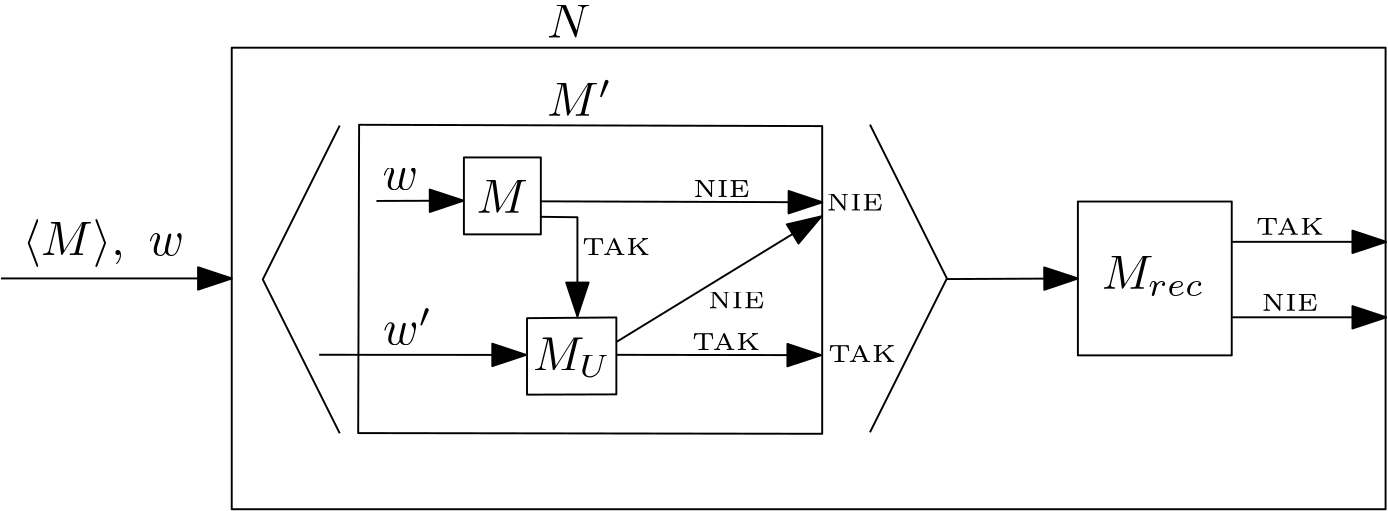
\includegraphics[width=0.75\linewidth]{img/Lrec.png}
    \end{figure}
    Jeśli \( w \in L(M) \), to \( M' \) akceptuje język nierekurencyjny (dlaczego?), a jeśli \( w \notin L(M) \), to \( L(M') = \emptyset \in R \). Zatem \( N \) rozpoznaje język \( \overline{L_U} \), co prowadzi do sprzeczności.
\end{proof}

\begin{theorem}
    \( L_{nrec} \notin \re \)
\end{theorem}
\begin{proof}
    Załóżmy dla dowodu nie wprost, że \( L_{nrec} \in \re \). Konstruujemy maszynę \(N\):
    \begin{figure}[H]
        \centering
        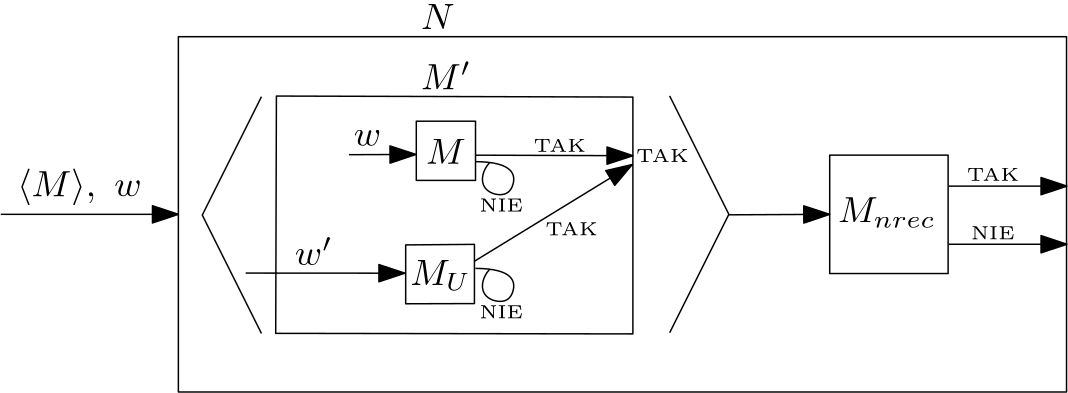
\includegraphics[width=0.75\linewidth]{img/Lnrec.png}
    \end{figure}
    Symulujemy na zmianę po jednym kroku \( M \) i \( M_U \). Jeśli \( M \) akceptuje \( w \), to maszyna \( M' \) akceptuje wszystko, niezależnie od \( M_U \), a wtedy \( L(M') = \Sigma^* \), czyli nie jest nierekurencyjny, bo maszyna, która akceptuje wszystko bez dodatkowych obliczeń ma własność STOP. \\
    Jeśli \( w \notin L(M) \), to wynik \( M' \) zależy jedynie od \( M_U \), więc jest językiem nierekurencyjnym. Zatem \( N \) rozpoznaje język \( \overline{L_U} \), co prowadzi do sprzeczności.
\end{proof}